\section{Experimental Evaluation}

\subsection{Experimental setup} \label{subsec:setup}

Our data set consists of 148 process descriptions annotated by a biologist. The annotator was presented with annotation guidelines, annotated 20 descriptions and then annotations were discussed with the authors, after which all process descriptions were annotated. After training a second biologist, we measured inter-annotator agreement on 30 random process descriptions, resulting in agreement $\kappa=0.69$. 

Process descriptions were parsed with Stanford constituency and dependency parsers \cite{Klein03,Marneffe06}, and 35 process descriptions were set aside as a test set (\# of training set trigger pairs: 1932, \# of test set trigger pairs: 906). We performed 10-fold cross validation over the training set for feature selection and tuning of constraint parameters. For each constraint type (connectivity, chain-structure, and five triangle constraints) we introduced a parameter and tuned the seven parameters by coordinate-wise ascent, where for hard constraints a binary parameter controls whether the constraint is used, and for soft constraints it controls reward/penalty ($\alpha_k$).

We test the following systems: (a) \emph{All-Prev}: since the most common process structure is a chain of consecutive events we simply predict \textsc{Next} for every two adjacent triggers. (b) \emph{Local$_{base}$}: A pairwise classifier with features from previous work (Section~\ref{subsec:pairwise}) (c) \emph{Local} A pairwise classifier with all features (Section~\ref{subsec:pairwise-novel}) (d) \emph{Global}: Our full model that uses ILP inference.

%(d) \emph{Local$_{chain}$}: For every two adjacent triggers we pick the highest probability non-\textsc{None} relation using the local classifier. Again, this uses the assumption that many processes have a chain-structure.

To evaluate system performance we compare its set of predictions on all trigger pairs to the gold standard annotations and compute micro-averaged precision, recall and F$_1$. We perform two types of evaluations: (a) \emph{Full}: evaluation on our full set of 11 relations (b) \emph{Temporal:} Evaluation on temporal relations only, by collapsing \textsc{Previous}, \textsc{Causes}, and \textsc{Enables} to a single category and similarly for \textsc{Next}, \textsc{Caused}, and \textsc{Enabled} (inter-annotator agreement $\kappa=0.75$). We computed statistical significance of our results with the paired bootstrap resampling method \cite{efron1993}.

\subsection{Results} \label{subsec:results}

\begin{table}[t]
{\footnotesize
\begin{tabular}{| l | c | c | c | c | c | c |}
\hline
    & \multicolumn{3}{c|}{\textbf{Temporal}} & \multicolumn{3}{c|}{\textbf{Full}} \\
    & P & R & F$_1$ & P & R & F$_1$ \\
\hline
\hline
\emph{All-Prev} & 62.2 & 58.3 & 60.2 & 34.1 & 32.0 & 33.0 \\
%\emph{Local$_{base}$} & 65.7 & 49.6 & 56.5 &  51.7 & 39.0 & 44.5\\
\emph{Local$_{base}$} & 65.6 & 55.3 & 60.0 &  52.1 & 43.9 & 47.6\\
\emph{Local} & 66.2 & 58.3 & 62.0 & 54.7 & 48.3 & 51.3 \\
%\emph{Local} & 50.3 & \textbf{67.8} & 52.6 & 59.3 & \textbf{57.6} & 44.7 \\
%\emph{Local$_{chain}$} & 65.0 & 60.1 & 62.9 & 52.8 & 49.6  & 51.1 \\
\emph{Global} & \textbf{66.5} & \textbf{64.5*} & \textbf{65.5*} & \textbf{55.7} & \textbf{54.0*} & \textbf{54.8*} \\
\hline
\end{tabular}}
\caption{Test set results on all experiments. Asterisk (*) denotes statistical significance ($p<0.01$) against all other baselines.}
\label{tab:results}
\end{table}


\begin{figure*}[t]
\centering
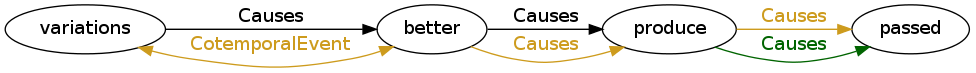
\includegraphics[width=0.9\textwidth]{figures/p144.png} 
\caption{Process graph example. Black edges are predictions of \emph{Local}, green edges indicate edges added by \emph{Global}, and gold edges represent gold standard edges. \textbf{Original text:} ``... Individuals in a population exhibit \emph{variations} in their heritable traits, and those with traits that are \emph{better} suited to their environment tend to \emph{produce} more offspring than those with traits that are not as well suited. In genetic terms, we now know that selection results in alleles being \emph{passed} to the next generation in proportions that differ from those in the present generation."}
\label{fig:graph}
\end{figure*}



Table~\ref{tab:results} presents performance of all systems. Our main result is that using global constraints improves performance on all measures in both full and temporal evaluations. Particularly, in the full evaluation recall improves by 12\% and overall F$_1$ improves significantly by 3.5 points against \emph{Local} ($p<0.01$). Recall improvement suggests that modeling connectivity allowed \emph{Global} to add correct relations in cases where some events were not connected to one another [double penalization? for now not mentioning it]

The full \emph{Local} classifier substantially outperforms \emph{Local$_{base}$}. This indicates that our novel features (Section~\ref{subsec:pairwise-novel}) are important for discriminating between process relations. Specifically, in the full evaluation \emph{Local} improves precision more than in the temporal evaluation, suggesting that designing syntactic and semantic features for connectives is useful for distinguishing \textsc{Next}, \textsc{Causes}, and \textsc{Enables} when the amount of training data is small.

The \emph{All-Prev} baseline performs quite badly in the full evaluation, but in temporal evaluation it performs reasonably well. This shows a strong tendency of process descriptions to proceed linearly from one event to the other, which is a general property of discourse structure \cite{schegloff73}.

Table~\ref{tab:degree} presents the degree distribution of \emph{Local} and \emph{Global} on the development set comparing to the gold standard. Clearly, degree distribution of \emph{Global} is much more similar to the gold standard than \emph{Local}. In particular, the connectivity constraint ensures that there are no isolated nodes and shifts mass from nodes with degree $0$ and $1$ to nodes with degree $2$.

%Table~\ref{} is a confusion matrix showing that it is hard to distinguish Causes, PrevEvent, and Cotemporal. These are not handled by global constraints and to handle this need other types of information.

\subsection{Analysis and Discussion} \label{subsec:analysis}

Table~\ref{tab:paramtuning} shows the order in which global constraints were introduced into the model using coordinate ascent on the development set. Connectivity is the first constraint to be introduced, and improves performance considerably. The chain constraint, on the other hand, is included last, which can be explained by examining the distribution of degrees in Table~\ref{tab:degree}. The predictions of \emph{Local} do not have many nodes with degree $>2$ and thus the effect of this constraint is small. As for triangle constraints, we see that three constraints are included in the model but two are discarded, since the changes they caused to the final solution did not improve F$_1$ on the development set.

\begin{table}[t]
{\footnotesize
\begin{tabular}{| l | c | c | c |}
\hline
    \textbf{Order} & \textbf{Parameter name} & \textbf{Value} ($\alpha$)& \textbf{F$_1$ score} \\
\hline
\hline
- & \emph{Local model} & - & 49.9 \\
1 & Connectivity constraint & $\infty$ & 51.2 \\
2 & \textsc{Same} transitivity &  0.5 & 52.0 \\
3 & \textsc{Cause}-\textsc{Cotemp} & 0.75 & 52.2\\
4 & \textsc{Same} contradiction & $\infty$ & 52.4\\
5 & Chain constraint & 0.25 & 52.5\\
\hline
\end{tabular}}
\caption{Order in which constraint parameters were set using coordinate ascent on the dev set. For each parameter, the value chosen and F$_1$ score after including the constraint are provided. A value of $\infty$ indicates a hard constraint}
\label{tab:paramtuning}
\end{table}

Figure~\ref{fig:graph} shows an example where the global constraints improve the predictions made by the local model. We see that the connectivity constraints help to identify the relation between \emph{produce} and \emph{passed} [TEMP EXAMPLE - FIND MORE INTERESTING]
